\documentclass{standalone}

\usepackage{times}
\usepackage{amsmath}
\usepackage{amssymb}

\usepackage[dvipsnames]{xcolor}
\usepackage{tikz}
\usetikzlibrary{arrows,arrows.meta,backgrounds,scopes}
\pgfdeclarelayer{background}
\pgfdeclarelayer{foreground}
\pgfsetlayers{background, main, foreground}

\usepackage{pgfplots}
\pgfplotsset{compat=1.15}
\begin{document}
	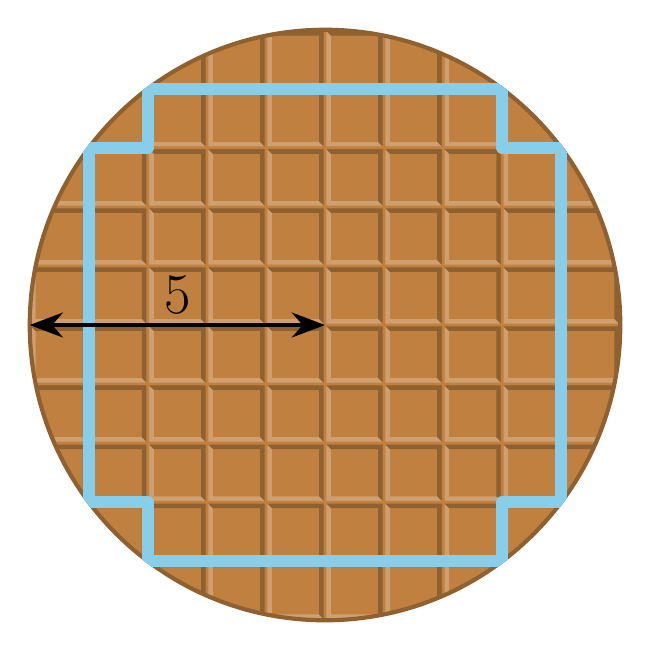
\begin{tikzpicture}[x=0.75cm,y=0.75cm]
		\newcommand{\drawCell}[2]{
			\fill[brown] (#1,#2) rectangle (#1+1,#2+1);
			\fill[brown!75] (#1,#2+1) -- (#1+0.1,#2+0.9) -- (#1+0.1,#2+0.1) -- (#1+0.9,#2+0.1) -- (#1+1,#2) -- (#1,#2) -- cycle;
			\fill[brown!75!black] (#1,#2+1) -- (#1+0.1,#2+0.9) -- (#1+0.9,#2+0.9) -- (#1+0.9,#2+0.1) -- (#1+1,#2) -- (#1+1,#2+1) -- cycle;
		}
		\newcommand{\waffle}[1]{
			\begin{scope}[transparency group,opacity=1]
				\begin{scope}
					\clip (0.5*#1, 0.5*#1) circle (0.5*#1);
					\foreach \y in {0,...,#1}{
						\foreach \x in {0,...,#1}{
							\drawCell{\x}{\y}
						}
					}
					\draw[brown,line width=1] (0,0) grid[step=1] (#1+1,#1+1);
				\end{scope}
				\draw[brown!75!black,line width=1.5] (0.5*#1, 0.5*#1) circle (0.5*#1);
			\end{scope}
			\begin{pgfonlayer}{foreground}
				\draw[<->,>={Stealth[length=12]}, line width=1.5] (0,0.5*#1) -- (0.5*#1,0.5*#1) node[midway,above]{\huge\pgfmathparse{0.5*#1}\pgfmathprintnumber{\pgfmathresult}};
			\end{pgfonlayer}
		}
		\waffle{10}
		
		\clip (5, 5) circle (3.75cm+0.75pt);
		\draw[SkyBlue,line width=0.15cm,line join=round] (1,2) -- (2,2) -- (2,1) -- (8,1) -- (8,2) -- (9,2) -- (9,8) -- (8,8)-- (8,9) -- (2,9) -- (2,8) -- (1,8) -- cycle;
	\end{tikzpicture}
\end{document} 
